%!TEX root = ../../prace.tex

\section{Inventář}

Inventář se vyvolá klávesou \textbf{E}. Zobrazí se následující obrazovka:

\begin{figure}[!ht]\centering
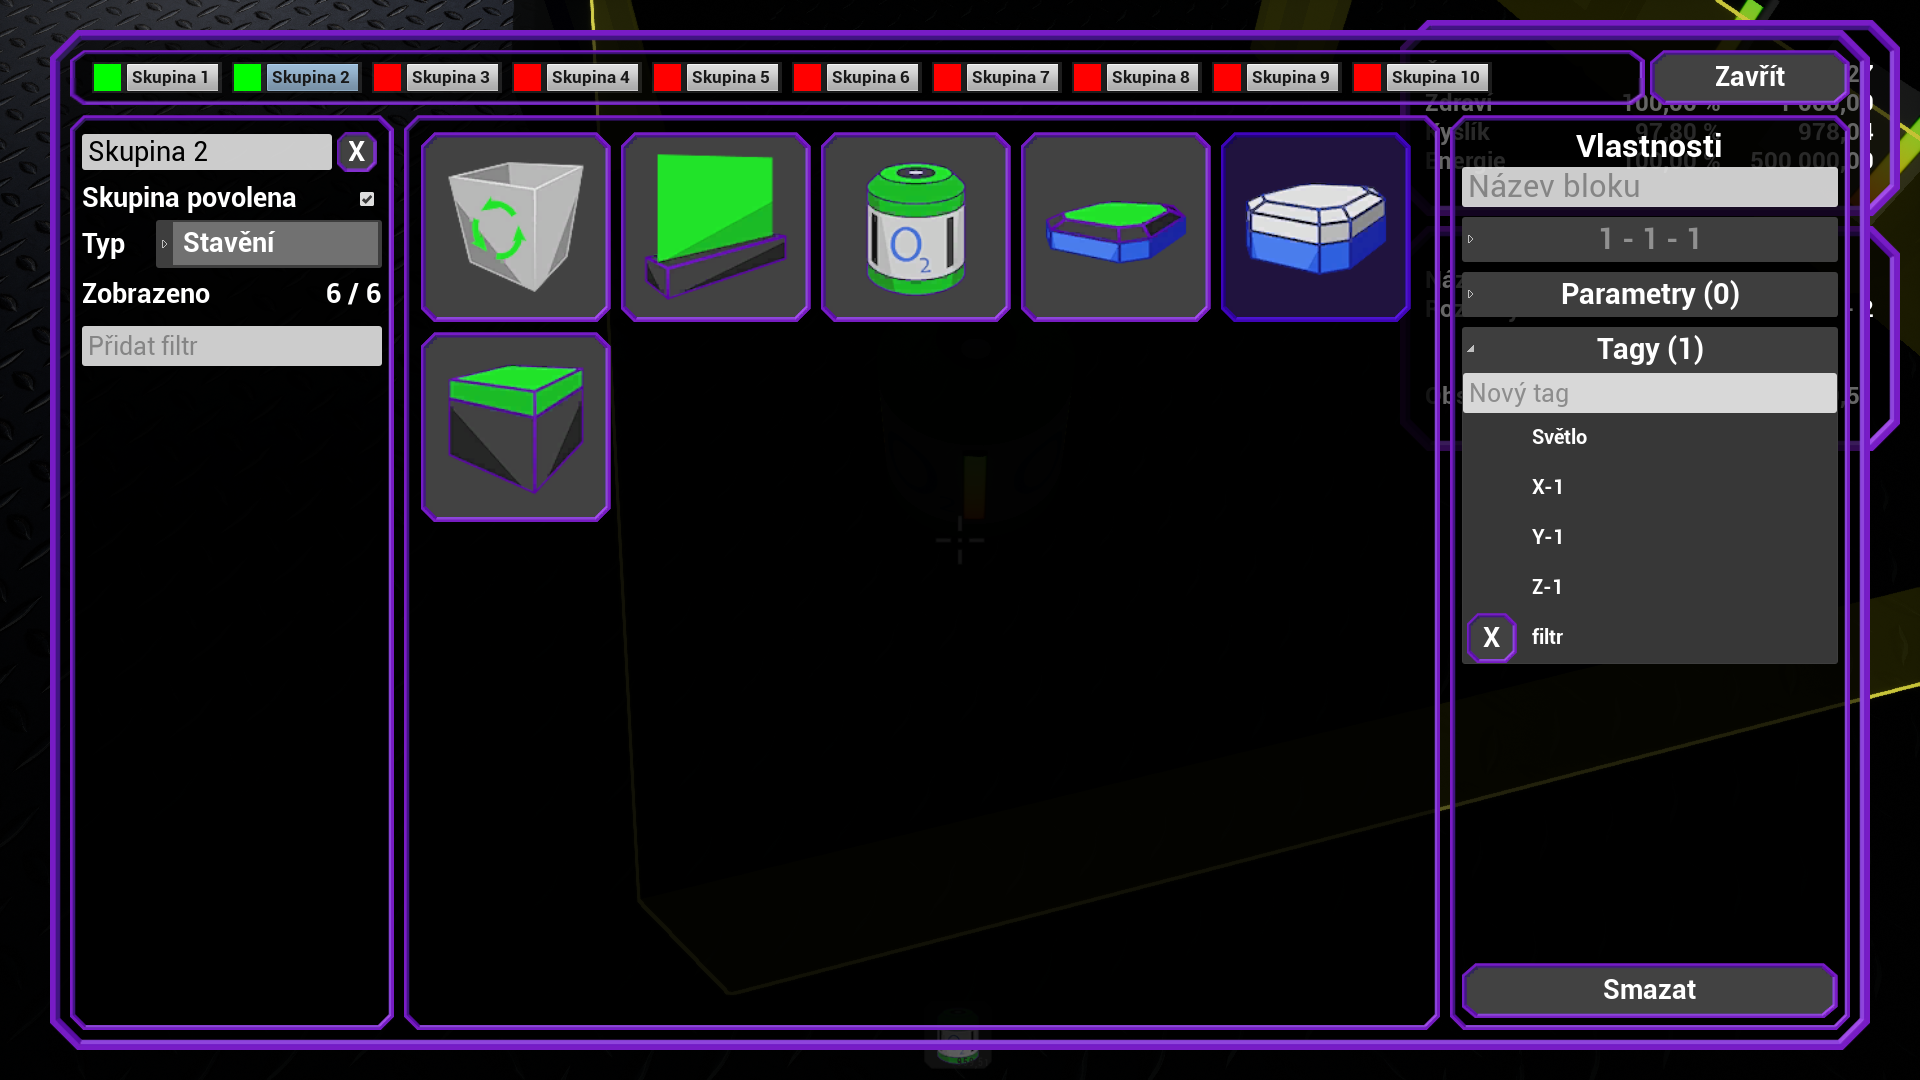
\includegraphics[ width=140mm]{../img/user/inventory/0AddTag}

\caption{Inventář -- přehled}
\label{fig:user_inventory_0AddTag}

\end{figure}

\FloatBarrier

V horní části je výběr skupin. Je možné vybírat z~10 skupin, které si lze pojmenovat dle libosti. Dále je možné je (de)aktivovat buď kliknutím na zelený / červený čtverec, nebo skrze příslušný checkbox v~editaci skupiny.
Je možné používat standardní změnu skupiny klávesami \textbf{ú} a~\textbf{)}, editační okno se pak příslušným způsobem změní. 

V \textit{levé} části je \textbf{editor skupiny}, jehož funkce budou popsány v~textu dále. \textit{Uprostřed} je možné vidět postavitelné či umístitelné položky, které jsou dofiltrovány dle právě nastaveného filtru. Výběrem položky lze editovat její vlastnosti v~\textit{pravé} části okna

\FloatBarrier

Každá skupina umožňuje definovat své filtry. Matematicky bychom mohli popsat filtrování jako vyhodnocení formule v~\textit{CNF}. Pokud do pole \textit{Přidat filtr} napíšeme tagy oddělené mezerou, do skupiny se přidá \textbf{nová} skupina s~výchozím pojmenováním.

\begin{figure}[!ht]\centering
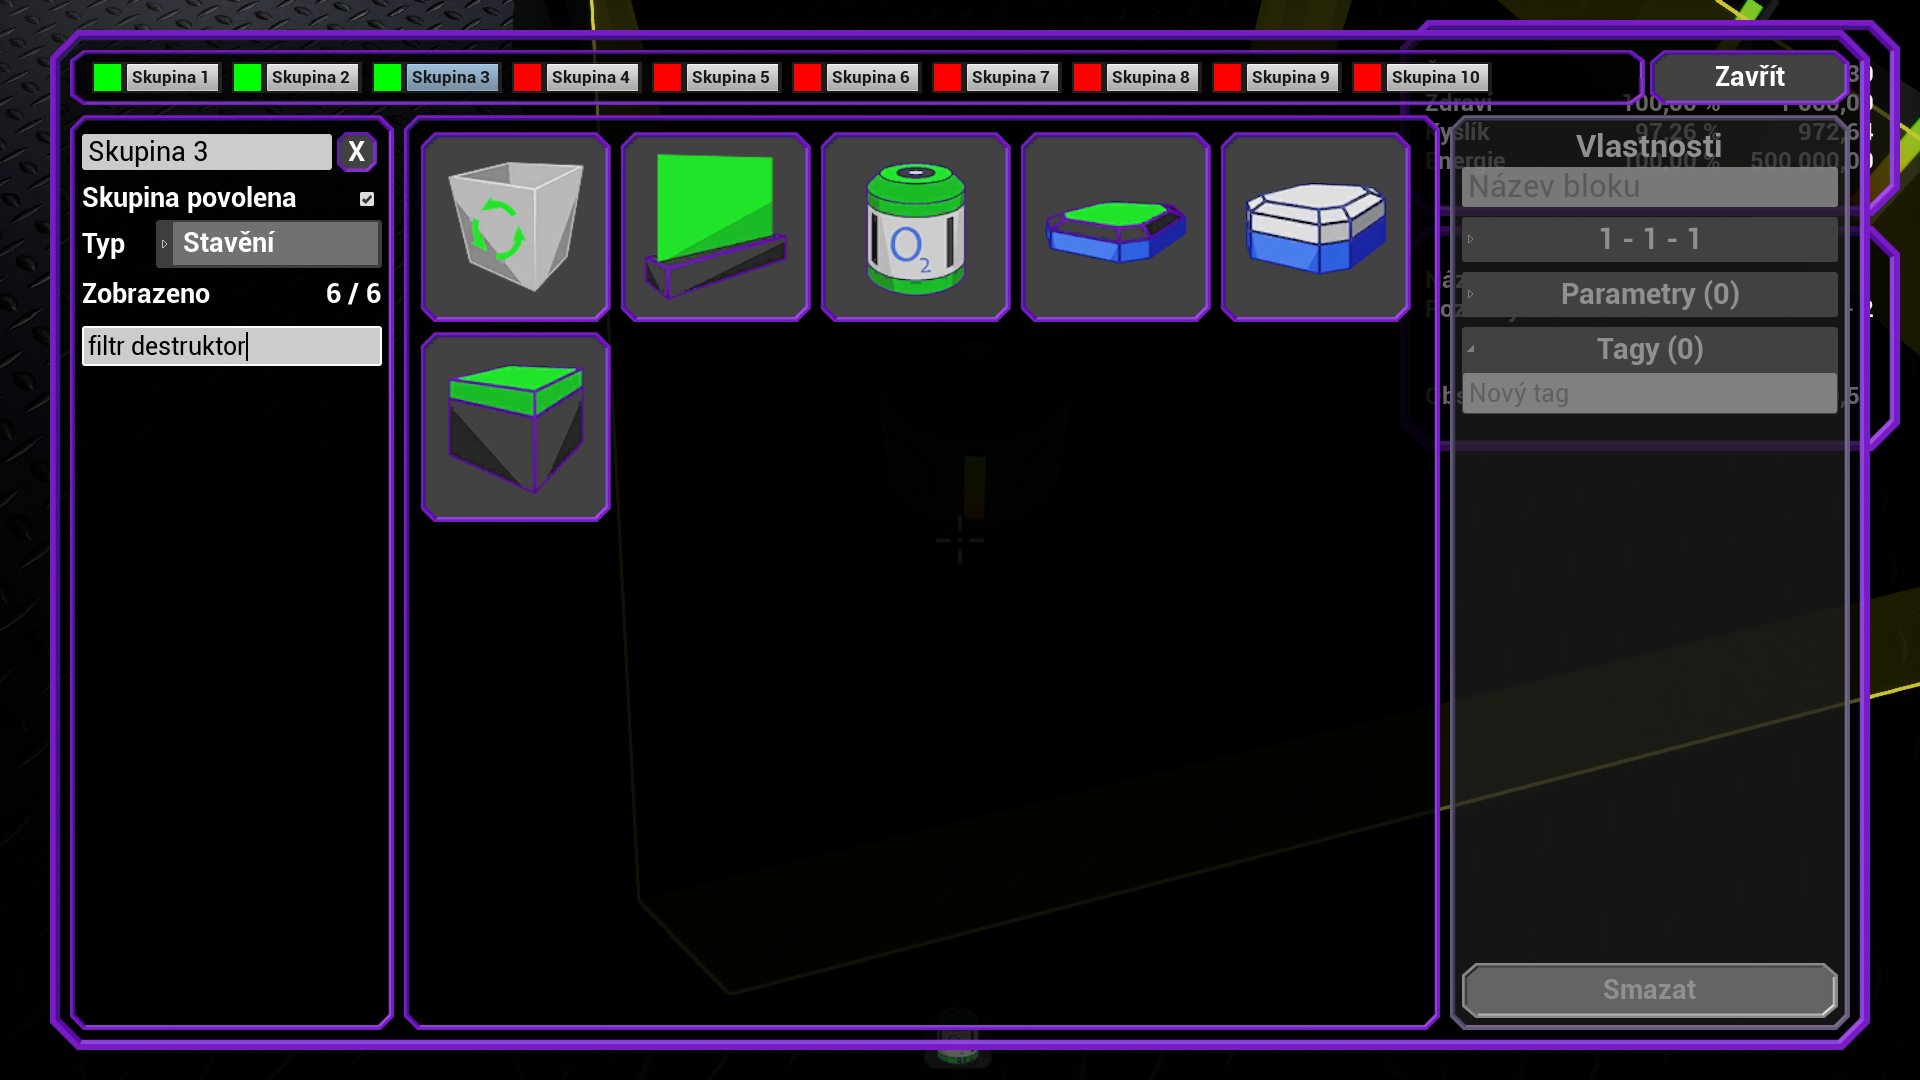
\includegraphics[ width=140mm]{../img/user/inventory/1setFilter}

\caption{Inventář -- přidání skupiny}
\label{fig:user_inventory_1setFilter}

\end{figure}

\FloatBarrier

Po přidání se seznam dostupných prvků dofiltruje podle nastavených tagů -- ve výsledku bude každá položka splňovat alespoň jeden tag z~každé skupiny. Shoda nemusí být přesná, tag objektu musí obsahovat podřetězec definovaný filtrem.
\begin{figure}[!ht]\centering
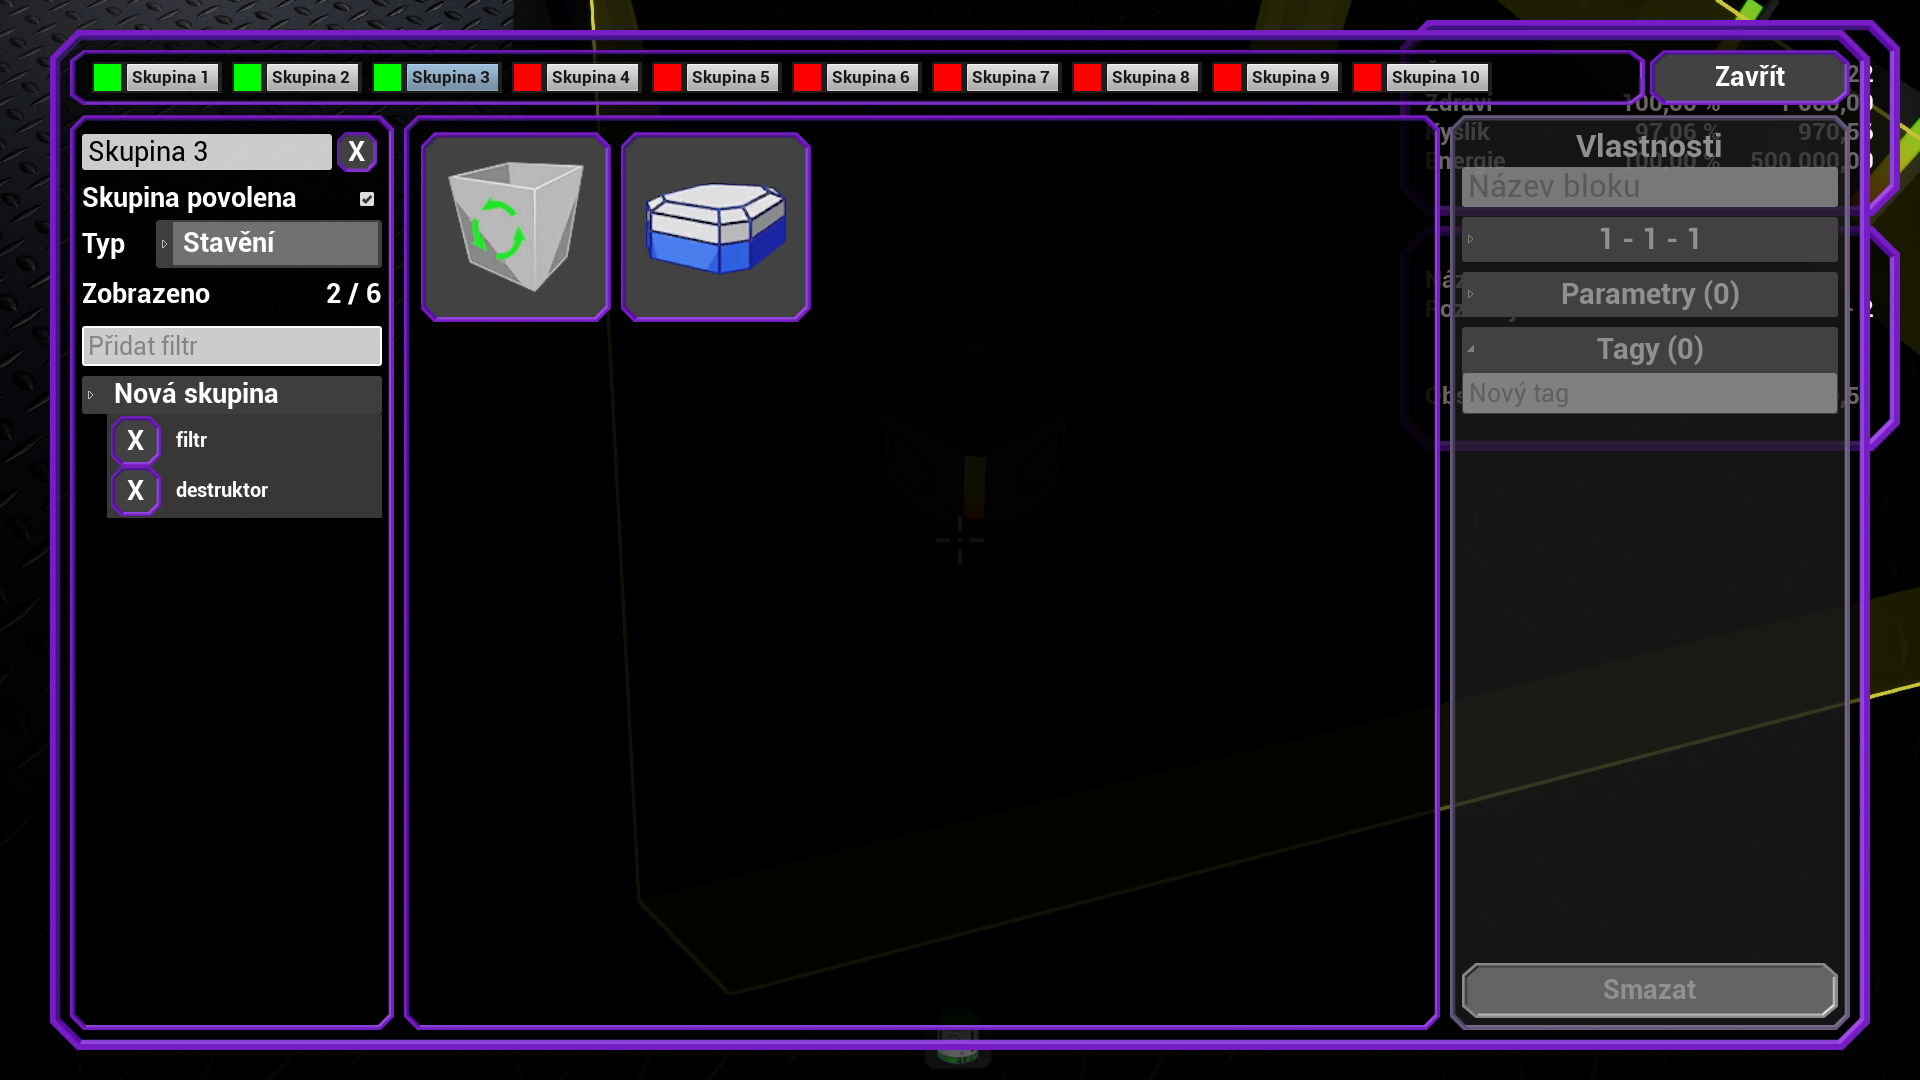
\includegraphics[ width=140mm]{../img/user/inventory/2filterResult}

\caption{Inventář -- výsledek s~filtrovanými položkami}
\label{fig:user_inventory_2filterResult}

\end{figure}

\FloatBarrier

Na následujícím obrázku je možné vidět filtry s~rozbalenými vlastnostmi. Zaměřme se nyní na část \textit{Nesbalovat}. Po zaškrtnutí této volby je zobrazena pouze hlavička skupiny.

\begin{figure}[!ht]\centering
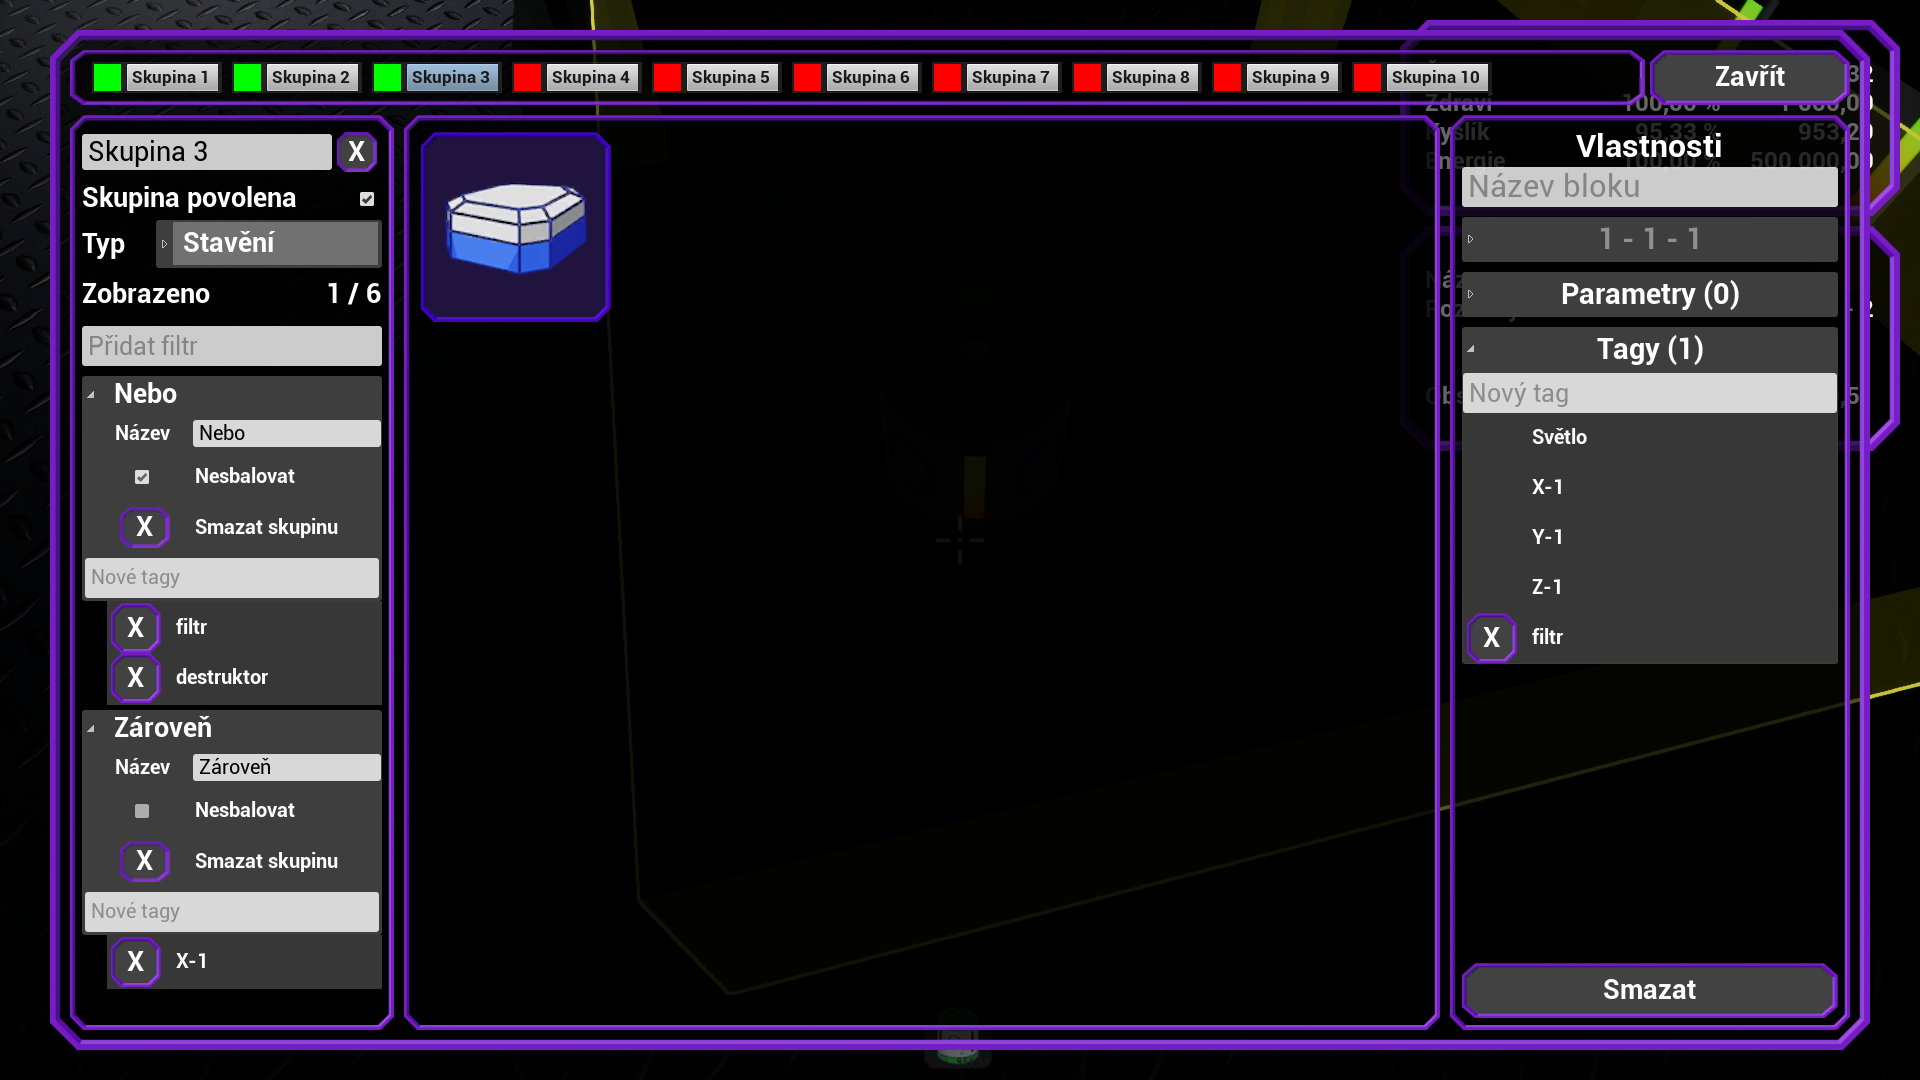
\includegraphics[ width=140mm]{../img/user/inventory/3additionalFilter}

\caption{Inventář -- Nová hra}
\label{fig:user_inventory_3additionalFilter}

\end{figure}

\FloatBarrier

Výsledný seznam se sbalenými vlastnostmi filtru:

\begin{figure}[!ht]\centering
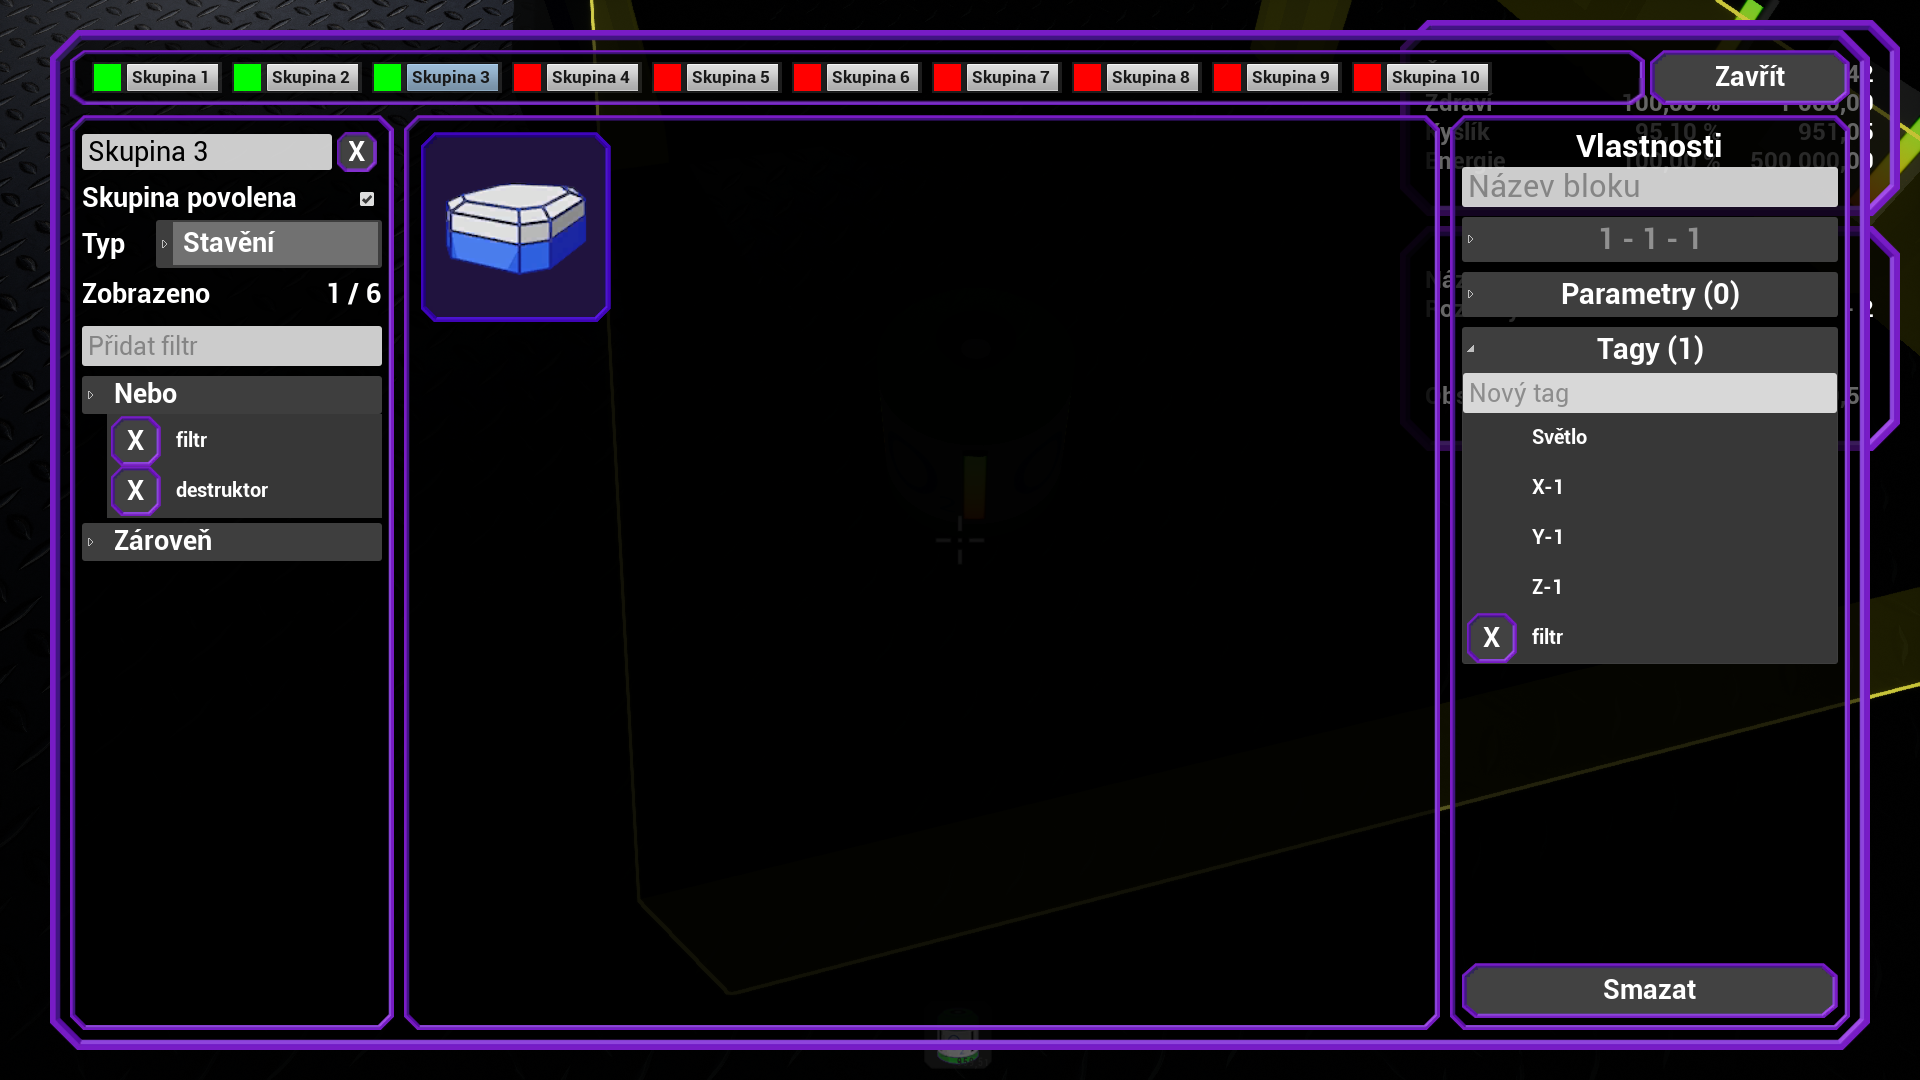
\includegraphics[ width=140mm]{../img/user/inventory/4addFilterCollapsed}

\caption{Inventář -- Nahrát hru}
\label{fig:user_inventory_4addFilterCollapsed}

\end{figure}

\FloatBarrier

Označené položky je také možné smazat z~inventáře. Umístitelné položky tak mohou být reálně zničeny. 

\begin{figure}[!ht]\centering
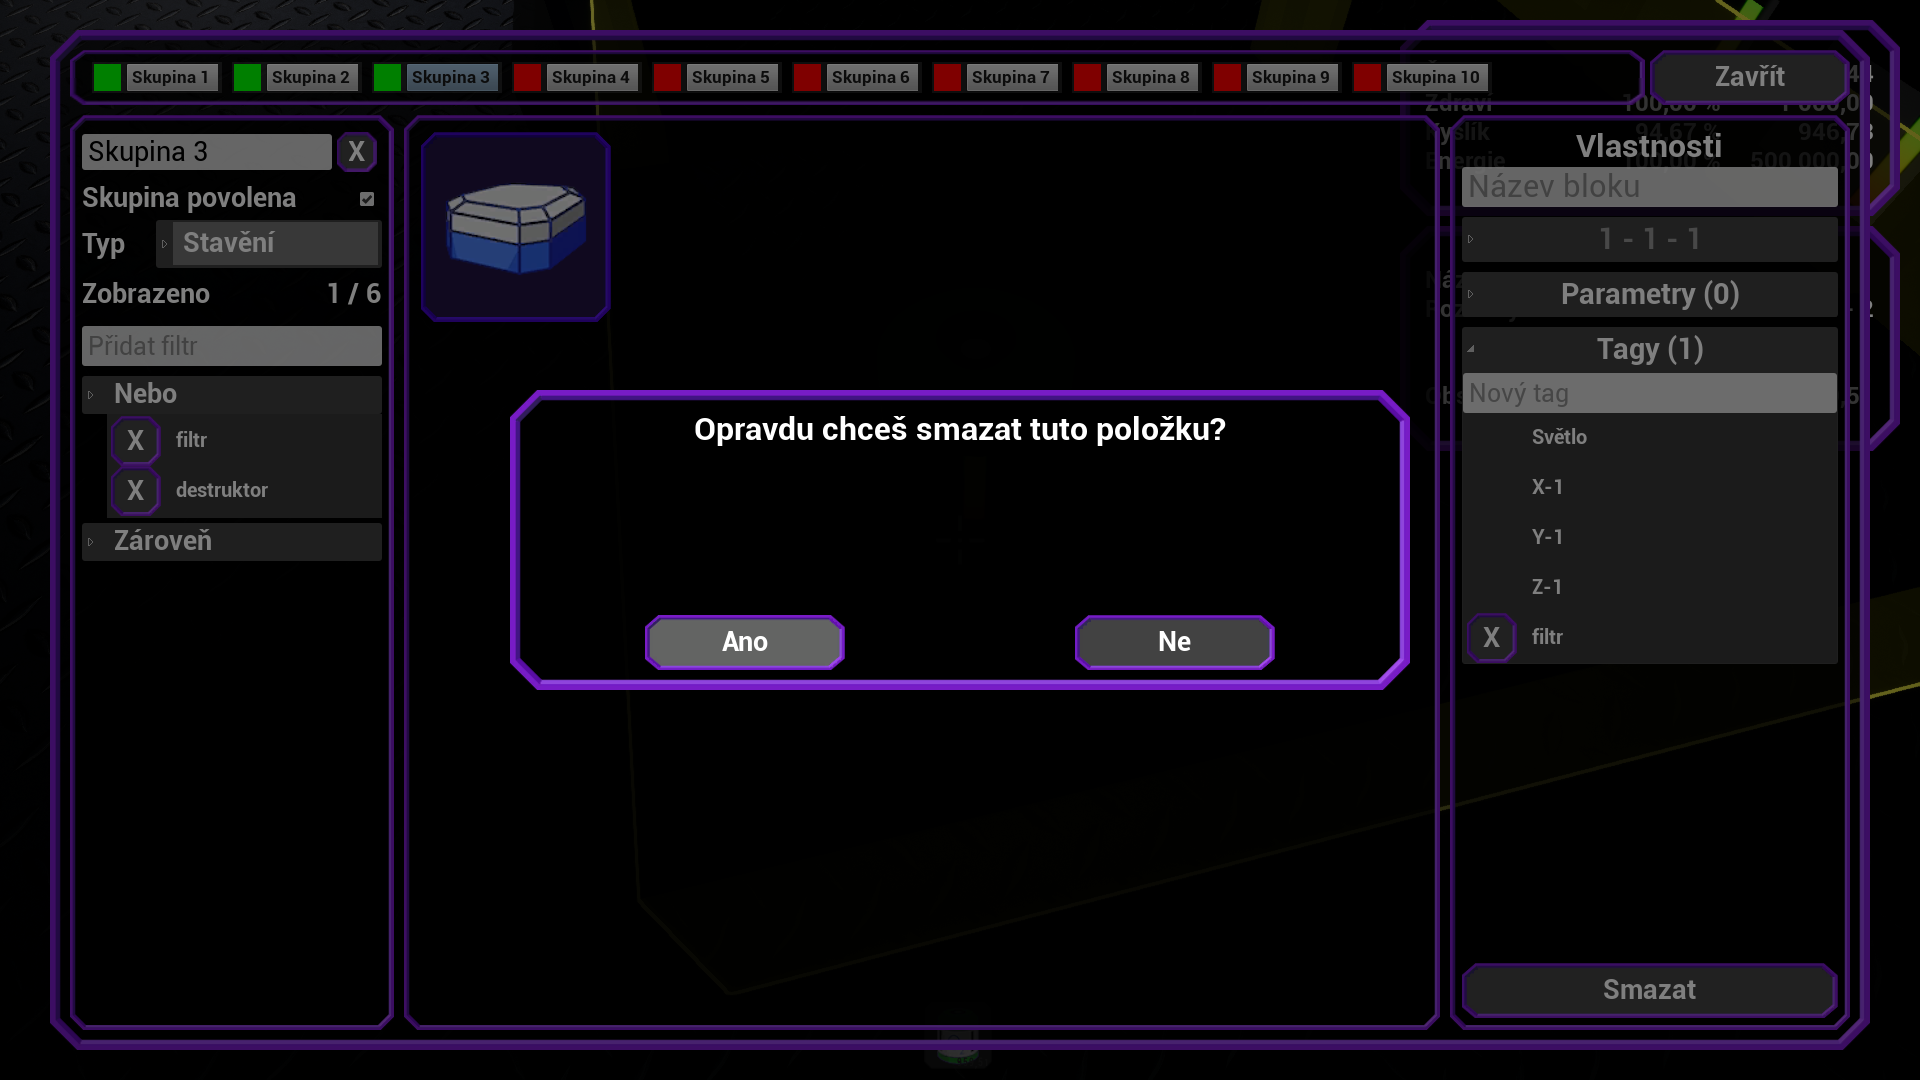
\includegraphics[ width=140mm]{../img/user/inventory/5deleteItem}

\caption{Inventář -- Nastavení}
\label{fig:user_inventory_5deleteItem}

\end{figure}

\FloatBarrier
V případě, že je zvolena položka s~dodatečnými parametry, je možné jejich hodnoty vidět v~editoru vlastností bloku

\begin{figure}[!ht]\centering
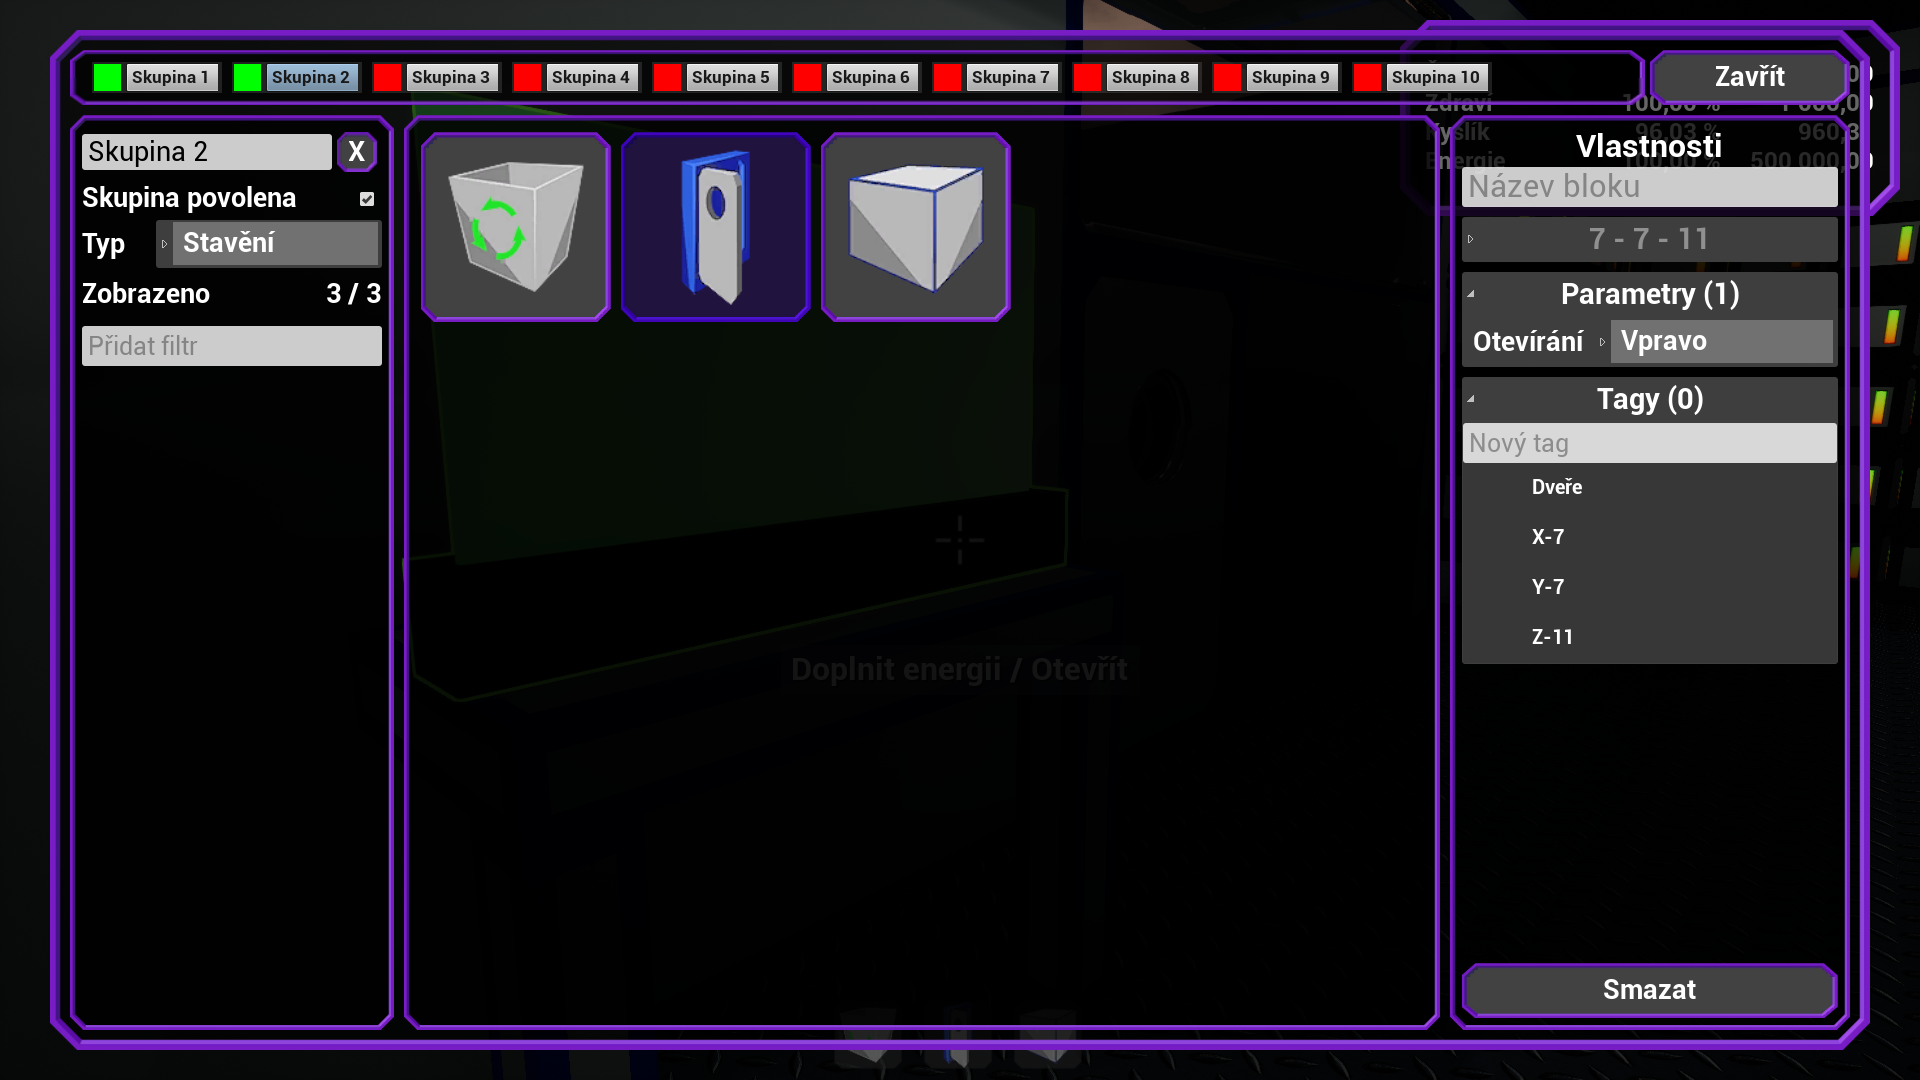
\includegraphics[ width=140mm]{../img/user/inventory/6itemWithParams}

\caption{Inventář -- Nastavení}
\label{fig:user_inventory_6itemWithParams}

\end{figure}


\FloatBarrier